\documentclass{../../presentation}

\title{PSE – Vorkurs Tag 3}
\author{Linus, Philipp, Tillmann, Tobias}
\institute{FIUS - Fachgruppe Informatik Universität Stuttgart}
\date{08.09.2025}

\makeatletter
\renewcommand{\lecture@pathprefix}[1]{../../logos/}
\makeatother

\usepackage{todonotes}
\setuptodonotes{inline}
\usepackage{tikz}
\usetikzlibrary{tikzmark}



\begin{document}

\begin{frame}
	\titlepage
\end{frame}

\begin{frame}
	\listoftodos
\end{frame}


\begin{frame}[fragile]
	\frametitle{Recap Tag 2 - Bedingungen \& Booleans}

	\begin{itemize}
		\item\pause Boolean: Wahrheitswerte \texttt{true} und \texttt{false}
		\item\pause Vergleiche: \texttt{==}, \texttt{!=}, \texttt{<}, \texttt{>}, \texttt{<=}, \texttt{>=}
		\item\pause Logische Operatoren: \texttt{\&\&} (UND), \texttt{||} (ODER), \texttt{!} (NICHT)
		\item\pause \textbf{\texttt{if}, \texttt{else}, \texttt{else if}} zur Entscheidungslogik
		      \begin{minted}[fontsize=\footnotesize]{java}
if (x > 5 && x < 10) {
  System.out.println("x ist zwischen 5 und 10");
} else {
  System.out.println("x ist außerhalb");
}
          \end{minted}
	\end{itemize}
\end{frame}


\begin{frame}[fragile]
	\frametitle{Recap Tag 2 - Schleifen}

	\begin{itemize}
		\item\pause \texttt{while}-Schleife: läuft, solange Bedingung \texttt{true} ist
		      \begin{minted}[fontsize=\footnotesize]{java}
while (!eingabe.equals("ok")) {
  eingabe = scanner.nextLine();
}
          \end{minted}
		\item\pause \texttt{for}-Schleife: Zählergesteuerte Schleife
		      \begin{minted}[fontsize=\footnotesize]{java}
for (int i = 0; i < 5; i++) {
  System.out.println(i);
}
          \end{minted}
		\item\pause \textbf{\texttt{break}}: beendet Schleife vorzeitig

	\end{itemize}
\end{frame}



\begin{frame}[fragile]
	\frametitle{Angenommen \dots}
	\begin{itemize}
		\item\pause Notendurchschnitt von zwei Studis berechnen
		      \begin{minted}{java}
            // Melanie
            double m1 = 1.7, m2 = 2.3, m3 = 1.3;
            double melanieDurchschnitt = (m1 + m2 + m3) / 3;
            System.out.println("Melanies Schnitt: " + melanieDurchschnitt);

            // Paul
            double p1 = 4.0, p2 = 2.3, p3 = 3.3;
            double paulDurchschnitt = (p1 + p2 + p3) / 3;
            System.out.println("Pauls Schnitt: " + paulDurchschnitt);
        \end{minted}
		      \begin{ausgabe}
			      Melanies Schnitt: 1.7666666666666666

			      Pauls Schnitt: 3.1999999999999997
		      \end{ausgabe}
	\end{itemize}
\end{frame}

\begin{frame}[fragile]
	\frametitle{Warum so nicht?!}
	\begin{itemize}
		\item\pause \textbf{Redundanz:} Gleicher Code mehrfach
		\item\pause \textbf{Fehleranfällig:} Zahlendreher möglich
		\item\pause \textbf{Schlecht wartbar:} Änderungen mehrfach nötig
		\item\pause \textbf{Nicht wiederverwendbar:} Nur an dieser Stelle nutzbar
		\item\pause \textbf{Unübersichtlich:} Logik geht unter
	\end{itemize}
	\vspace{2em}
	\begin{minipage}{\textwidth}
		\centering
		\onslide\pause{\Huge $\rightarrow$~}%
		\onslide{\Large Funktionen ermöglichen Wiederverwendung von Code!}
	\end{minipage}
\end{frame}

\begin{frame}[fragile]
	\frametitle{Was sind eigentlich Funktionen?}
	\begin{itemize}
		\item\pause  Möglichkeit Code auszulagern
		\item\pause Syntax:
		      \begin{minted}{java}   
Rückgabedatentyp Funktionsbezeichner(Datentyp Parametername,...){
        ...
        return Rückgabewert;
 }
        \end{minted}
		\item\pause in unserem Fall:
		      \begin{minted}[fontsize=\footnotesize]{java}
        static void avg(String name, double note1, double note2, double note3) {
            double avg = (note1 + note2 + note3) / 3;
            System.out.println(name + "s Schnitt: " + avg);}
            \end{minted}
	\end{itemize}
	Schlüsselwort \texttt{static} ist hier notwendig wird in PSE genauer erklärt
\end{frame}


\begin{frame}[fragile]
	\frametitle{\texttt{return}}

	\begin{itemize}
		\item\pause Funktionen können Werte zurückgeben
		\item\pause z.B. eine Zahl:
		      \begin{minted}[escapeinside=||]{java}
static |{\tikzmark{rettyp}}|int add(int num1, int num2){
    int sum = num1 + num2;
    return sum;
}
\end{minted}
		\item\pause Datentyp des \texttt{return}-Werts muss im Funktionskopf stehen
		      \begin{tikzpicture}[remember picture, overlay]
			      \draw[->, red, thick]
			      ([yshift=2.5em,xshift=2.5em]pic cs:rettyp)
			      -- ([yshift=1.5ex,xshift=1.0em]pic cs:rettyp)
			      node[anchor=west, yshift=2.0em, xshift=1.0em] {\scriptsize hier \texttt{int} Rückgabetyp};
		      \end{tikzpicture}
		\item\pause Wenn kein Rückgabewert $\rightarrow$ \texttt{void} (wie vorhin)
	\end{itemize}
\end{frame}

\begin{frame}[fragile]
	\frametitle{Verwendung von \texttt{return}}

	\begin{itemize}
		\item\pause Rückgabewert wird zurück an den Aufrufer gegeben
		\item\pause Speicherung in Variable
		      \begin{minted}{java}
int result = add(3, 4);
System.out.println(result); 
		\end{minted}
		      \begin{ausgabe}
			      7
		      \end{ausgabe}
		\item\pause \texttt{return} beendet Funktion sofort
		\item\pause Code nach \texttt{return} wird nicht mehr ausgeführt
	\end{itemize}
\end{frame}


\begin{frame}[plain]
    \centering
    {\Huge\bfseries Code together: Promillerechner}

    \vspace{1em}

    \begin{flushleft}
        \textbf{Aufgabe:} Schreibe eine Methode \texttt{berechnePromille}, die anhand der Getränkemenge (in Litern), 
        des Alkoholgehalts (Vol-\%) und des Körpergewichts die Blutalkoholkonzentration berechnet. 

        \vspace{1em}

        \textbf{Formeln:} 
        \[
            \text{Promille} \approx \frac{\text{Alkohol in Gramm}}{\text{Körpergewicht in kg} \times 0{,}65}
        \]
        \[
            \text{Alkohol in Gramm} = \text{Getränkemenge in Liter} \times \text{Vol\%} \times 8
        \]
    \end{flushleft}
\end{frame}




\begin{frame}[fragile]{Die \texttt{main}-Funktion}
	\begin{itemize}
		\item\pause Einstiegspunkt jedes Java-Programms
		\item\pause Wird beim Start automatisch aufgerufen
		\item\pause Muss exakt so deklariert sein:
	\end{itemize}

	\vspace{0.5em}

	\begin{minted}[fontsize=\footnotesize]{java}
public static void main(String[] args) {
    // Hier beginnt das Programm
}
\end{minted}
\end{frame}


\begin{frame}[fragile]{Sichtbarkeit von Variablen (Scopes)}
	\begin{itemize}
		\item\pause Variablen sind sichtbar im aktuellen und in allen tieferen Blöcken
		      \begin{minted}[fontsize=\footnotesize]{java}
public static void main(String[] args) {
int y = 10;

if (y > 5) {
    System.out.println(y); // OK – Zugriff auf äußere Variable
}}
    \end{minted}
	\end{itemize}
\end{frame}

\begin{frame}[fragile]
	\frametitle{Sichtbarkeit von Variablen (Scopes)}
	\begin{itemize}
		\item\pause In äußeren Blöcken sind sie nicht sichtbar
		      \begin{minted}[fontsize=\footnotesize]{java}
public static void main(String[] args) {
    int x = 5;
}
public static void andereMethode() {
    System.out.println(x); // Fehler! x ist hier nicht sichtbar
}
    \end{minted}

		\item\pause Gilt für alle Blöcke: Funktionen, if, Schleifen, etc.
	\end{itemize}
	
\includegraphics[width=1\linewidth]{img/scopesmemehoriz.png}
\end{frame}


\begin{frame}[plain]
  \centering
  {\Huge\bfseries{Check Yourself!}}
\end{frame}

\begin{frame}[fragile]
  \frametitle{Frage 1: Was gibt die void-Deklaration bei einer Funktion an?}
  \begin{ausgabe}
    Die Funktion gibt keinen Wert zurück
  \end{ausgabe}
\end{frame}

\begin{frame}[fragile]
  \frametitle{Frage 2: Welche Aussage ist richtig?}
  \begin{minted}{java}
public static int multiply(int a, int b) {
    int result = a * b;
    return result;
}
  \end{minted}
  \begin{ausgabe}
    Es gibt keinen Fehler im Code
  \end{ausgabe}
\end{frame}

\begin{frame}[fragile]
  \frametitle{Frage 3: Bilde die erste Zeile einer Funktion, die eine Note als Parameter erhält und nichts zurückgibt?}
  \begin{minted}{java}
public static void printGrade(double grade) {
    // für Lösung nur Zeile 1 relevant
}

  \end{minted}
\end{frame}

\begin{frame}[fragile]
  \frametitle{Frage 4: Welche Aussage über Funktionen in Java ist richtig??}
  \begin{ausgabe}
    Methoden in Java können andere Methoden aufrufen
  \end{ausgabe}
\end{frame}

\begin{frame}[fragile]
  \frametitle{Frage 5: Was wird ausgegeben?}
  \begin{minted}{java}
if (true) {
    int y = 8;
}
System.out.println(y);

  \end{minted}
  \begin{ausgabe}
    Fehler
  \end{ausgabe}
\end{frame}

\begin{frame}[fragile]
  \frametitle{Frage 6: Was wird ausgegeben?}
  \begin{minted}{java}
int i = 0;
for (i = 0; i < 3; i++) {
    System.out.print(i);
}
System.out.print(i);
  \end{minted}
  \begin{ausgabe}
    0123
  \end{ausgabe}
  Was würde ausgegeben werden, wenn Zeile 1 entfernt wird?
\end{frame}

\begin{frame}[fragile]
  \frametitle{Frage 7: Was wird ausgegeben?}
  \begin{minted}{java}
public static void main(String[] args) {
    int a = 5;
    zeigeA(a);
    System.out.print(a);
}

public static void zeigeA(int a) {
    a = a + 1;
    System.out.print(a);
}
  \end{minted}
  \begin{ausgabe}
    65
  \end{ausgabe}
\end{frame}

\begin{frame}[fragile]
	\frametitle{Was ist ein Array?}
	\begin{itemize}
		\item\pause Arrays speichern mehrere Werte des selben Datentyps
		\item\pause Länge ist beim Erstellen fest und unveränderlich
		\item\pause Elemente sind geordnet und über einen Index erreichbar
		\item\pause Syntax:
		      \begin{minted}{java}
        Datentyp[] Bezeichner = new Datentyp[ArrayLänge];
    \end{minted}
		\item\pause z.B.: leeres Array für 5 Ganzzahlen
		      \begin{minted}{java}
		int[] numbers = new int[5];
	\end{minted}
	\end{itemize}
\end{frame}

\begin{frame}[fragile]
	\frametitle{Zugriff auf Array-Elemente}
	\begin{itemize}
		\item\pause Jedes Element hat einen Index
		\item\pause über Index lässt sich auf Elemente zugreifen
	\end{itemize}
	\begin{columns}
		\column{0.5\linewidth}
		\begin{minted}{java}
            int[] numbers = new int[5];
            numbers[0] = 6;
            numbers[2] = 9;
        \end{minted}

		\column{0.5\linewidth}
		\begin{center}
			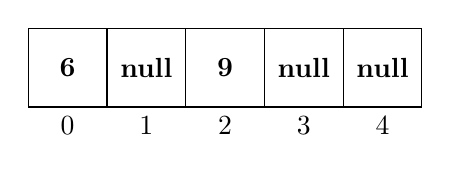
\begin{tikzpicture}
				\foreach \x in {0,1,...,4} {
						\draw (\x,0) rectangle coordinate(c\x) (\x+1, 1);
						\node[below] at (\x+0.5, 0) {\x};
					}
				\node at (c0) {\bf 6};
				\node at (c1) {\bf null};
				\node at (c2) {\bf 9};
				\node at (c3) {\bf null};
				\node at (c4) {\bf null};
			\end{tikzpicture}
		\end{center}
	\end{columns}

	\vspace{0.5cm}
	\begin{itemize}
		\item\pause Arrays können auch direkt mit Werten initialisiert werden
		      \begin{minted}{java}
    String[] grillSachen = {"würstchen", "steak", 
                            "grillkäse", "maiskolben"};
    \end{minted}
	\end{itemize}
\end{frame}

\begin{frame}[fragile]
	\frametitle{Arrays durchlaufen mit \texttt{.length}}
	\begin{itemize}
		\item\pause speichert Länge des Arrays
		      \begin{minted}{java}
			Bezeichner.length
		\end{minted}
		\item\pause damit lässt sich über alle Elemente iterieren
		      \begin{minted}{java}
    System.out.println(grillSachen[1]);
    for (int i = 0; i < grillSachen.length; i++) {
        System.out.println(grillSachen[i]);
    }
    \end{minted}
		      \begin{ausgabe}
			      steak \\
			      würstchen \\
			      steak \\
			      grillkäse \\
			      maiskolben
		      \end{ausgabe}
	\end{itemize}
\end{frame}

\begin{frame}[fragile]
    \frametitle{Ende}
    \begin{columns}
        \begin{column}{0.65\textwidth}
            \begin{itemize}
                \item Folien und Aufgaben: \newline \url{https://fius.de/index.php/pse-vk-folien/}
            \end{itemize}
        \end{column}
        \begin{column}{0.35\textwidth}
            \qrcode{https://fius.de/index.php/pse-vk-folien/}
        \end{column}
    \end{columns}

    \vspace{3em}

    \begin{columns}
        \begin{column}{0.65\textwidth}
            \begin{itemize}
                \item Feedback: \newline \url{\feedbackurl}
            \end{itemize}
        \end{column}
        \begin{column}{0.35\textwidth}
            \qrcode{\feedbackurl}
        \end{column}
    \end{columns}

    Wenn ihr Fragen habt, sagt Bescheid!

\end{frame}

\end{document}
